\chapter[A shim Layer for persistent memory]{A shim layer for persistent memory}

As we have discussed, the release of Intel Optane PMM opens a major opportunity for serverless storage services. This memory technology provides a unique combination of affordable larger capacity, high-performance, and support for data persistence \cite{IntelOp15:online}. When configured in App-Direct mode, the Optane DIMM and DRAM DIMMs act as independent memory resources under direct load/store control of the applications. This allows the Optane PMM capacity to be used as byte-addressable persistent memory that is mapped into the system application space and directly accessible by applications. Together, these advantages enable Optane PMM to be used as persistent storage with memory-like speeds.

Unfortunately, the resource contention observed within Optane PMM can impose serious performance and contractual implications for a multi-tenant serverless storage service. Given the hallmark autoscaling features of serverless computing, the memory’s limited ability to handle accesses from multiple threads can degrade the overall system’s performance when workload spikes occur. Furthermore, these storage systems make efficient use of their infrastructure by allowing multiple users, or tenants, to share the physical resources. The performance degradation caused by Optane PMM can lead tenants to experience significant performance variations. The latter inhibits service providers from offering certain service level agreements.

To reduce the contention effect, previous studies recommend limiting the number of threads that access Optane PMM simultaneously. In \cite{yang2020empirical}, Yang et. al they improve the performance of an NVM-aware file system by limiting the number of writer threads that access each Optane DIMM. Similarly, Ribbon \cite{wu2020ribbon} controls the number of threads performing CLF and adjusts this number dynamically at runtime. While this approach provides a viable solution, it introduces management problems for a system administrator of a multi-tenant serverless storage.

Given the complexity of serverless computing workloads, implementing efficient concurrency control mechanisms for optimizing an Optane-based serverless storage service is a challenging task. These challenges are discussed in section 3.1, but in short, service providers have three crucial tasks when implementing these control mechanisms. First, they must provide predictable performance, ensuring that all the SLAs from different workloads are met. Second, they must scale resources transparently to meet the current workload demand. Finally, they must come up with policies that allow their system to adapt quickly to sudden workload shifts. To this end, we propose a solution that takes on these responsibilities from the service providers.

In this work, we present a shim layer that addresses the shortcomings of Intel Optane PMM highlighted above, while meeting the different service level agreements from multiple tenants under shifting workloads. Our shim layer, called NVM Middleware, distinguishes between latency-critical and throughput-oriented workloads and applies different concurrency control mechanisms for each one. This enables the system to reduce the contention on the memory device, as well as the interference among workloads with different service level agreements. In addition, we propose the development of a reinforcement learning agent to adapt the NVM Middleware quickly to changing workloads. The agent takes into account the characteristics and service level agreements and learns from past experiences to scale resources accordingly.


\section{Motivation}
In this section, we discuss the pain points of controlling the number of threads to optimize Optane PMM within a serverless storage service and explain the design goals of the NVM Middleware.

\subsection{Concurrency Control Challenges in a serverless storage service}

When building an Optane PMM based serverless storage service, optimizing the memory's performance is just the start. Early works in serverless computing have identified several tasks that a storage service must perform efficiently to meet the demands of serverless computing \cite{180275,jonas2019cloud,klimovic2018understanding,klimovic2018pocket,wu2019autoscaling,romero2021faat}. As a result, service providers must ensure that their concurrency control policies do not interfere with these design goals. In this work, we focus on three challenges faced by service providers when designing a high-performance storage service based on Optane PMM.

\textbf{Support for a wide heterogeneity of applications.} In serverless computing, users typically deploy their applications as a collection of serverless functions that share data among them using remote storage. Previous studies suggest that these applications vary considerably in the way store, distribute, and process data. This diversity is reflected in multiple ways, such as data access size \cite{klimovic2018pocket,romero2021faat}, data access patterns \cite{romero2021faat}, and their performance requirements [180275,jonas2019cloud]. Therefore, service providers face the challenge of tuning the concurrency level to support many types of applications. In this work, we argue that considering the workload characteristics is key for tuning the system efficiently. The allocation of resources can vary depending on the workload type.

\textbf{Compliance with Service Level Agreements.} The success of a storage service relies on its ability to comply with various service level agreements (SLAs). SLAs play a critical role in governing the relationship between the storage provider and its customers. They help establish clear expectations between both parties regarding the quality of storage service. Therefore, service providers face the challenge of staying in compliance with these SLAs while they seek to optimize Optane PMM. 

\textbf{Automatic and transparent scaling.} Serverless workloads are extremely unpredictable. These workloads can launch hundreds of functions instantaneously to meet application demands \cite{klimovic2018understanding}. Furthermore, the data access patterns of the applications can change dramatically over time \cite{romero2021faat,wu2019autoscaling}. Service providers face the challenge of scaling the resources, such as number of threads, automatically to meet the demands of changing workloads. In addition, they must ensure that the system adapts quickly enough to avoid missing SLAs.


\subsection{NVM Middleware Design Overview}

We design NVM Middleware with three main design goals.

\textbf{Workload-aware Contention Management.} We focus our work on two main types of workloads: interactive and batch applications. Interactive applications, such as web-based platforms, enable real-time interactions between the user and the application. Low latency is critical to ensure that the user input is processed quickly, and feedback is delivered in real-time. On the other hand, batch applications, such as data analytics jobs, facilitate efficient processing of large-scale data. These workloads prioritize high throughput to process large volumes of data efficiently.

The NVM Middleware leverage insights about the workload characteristics, resource demands, and performance requirements of applications to make informed decisions about resource allocation and contention resolution. By dynamically adjusting resource allocation and contention resolution mechanisms based on the workload characteristics, the NVM Middleware mitigates contention-induced performance degradation and ensures efficient resource sharing among co-located applications. This adaptive approach enables the NVM Middleware to allocate resources judiciously to maximize overall system efficiency and meet diverse performance requirements of both interactive and batch applications. By using the content-aware contention management offered by the NVM Middleware, a storage system using Optane PMM can effectively balance the needs of different workload types, ensuring optimal performance and resources utilizing in multi-tenant environments.

\textbf{SLA-driven autoscaling policies.} The NVM Middleware leverages SLAs, which define the quality-of-service parameters agreed up between the service provider and their customers, to dynamically adjust contention resolution mechanisms in response to changes in service level agreement metrics. It continuously monitors SLA metrics, such as 99th latency and throughput, and evaluates its own performance against predefined SLA targets. This real-time monitoring allows the NVM Middleware to detect deviations from SLA requirements and triggers scaling actions to dynamically adjust resource allocation. By aligning resource provisioning with SLA requirements, the NVM Middleware can ensure a consistent and reliable performance from Optane PMM, even under dynamic workload changes.

\textbf{RL-driven autoscaling policies.} Besides leveraging SLAs to dynamically provision resources and adjust contention resolution mechanisms, our solution proposes the use of Reinforcement Learning to learn from past experiences and predict future behaviors.  These RL-driven policies enable the NVM Middleware to adapt to changing workload patterns over time and meet SLAs objectives more effectively than traditional threshold-based approaches []. Moreover, given the dynamic and unpredictable of serverless workloads, we propose a model-free algorithm, Q-Learning, to continuously learn the optimal policy based on observed experiences, allowing the NVM Middleware to adapt to new scenarios without needing to explicitly model them.

\section{Architecture}

\begin{figure}[ht]
  \centering
  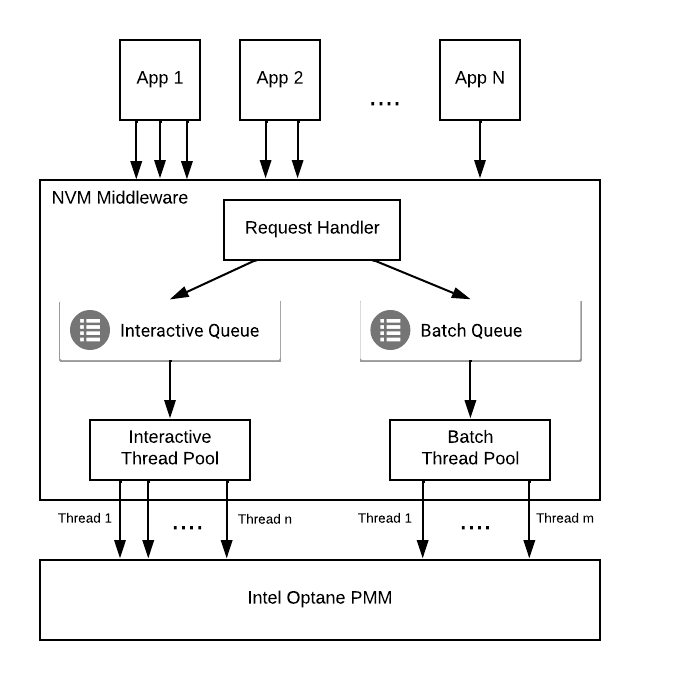
\includegraphics[scale=1]{images/nvm_design.png}
  \caption[NVM Middleware Architecture]{NVM Middleware Architecture}
  \label{fig:nvm_architecture}
\end{figure}

Figure \ref{fig:nvm_architecture} provides an overview of the NVM Middleware architecture. Positioned as a middle layer connecting user applications with Optane PMM, its design is tailored for seamless integration within a storage service, serving as an optimization layer specifically targeting Optane PMM. It comprises a request handler, two concurrency thread pools, and a monitoring and resource management module.

The request handler serves as the primary interface for handling user I/O requests. Upon receipt, it segregates requests into two distinct non-blocking First-In-First-Out (FIFO) queues: one tailed for latency-sensitive requests and the other for throughput-centric ones. Leveraging insights into workload characteristics, the handler intelligently allocates requests to the appropriate queue. Moreover, each queue is assigned a dedicated pool of worker threads tasked with dispatching I/O requests to Optane PMM using PMEMKV. Notably, these thread pools operate independently and are dynamically managed and scaled by the Reinforcement Learning agent to meet predetermined latency and throughput goals.

The Monitoring and Resource Management module offers an interface to monitor system load and SLA performance metrics. This module initiates a separate control thread tasked with gathering data on key parameters within the NVM Middleware, such as 99th latency, throughput, and system load. Utilizing this information, the RL agent makes data-driven decisions regarding optimal thread pool scaling. Subsequently, these decisions are communicated to the Monitoring and Resource Management module, which executes the required actions within the NVM Middleware.

\section{Programming Interface}

\begin{table}[ht]
  \centering
  \caption{Programming Interface}
  \label{table:programming_interface}
  % Tabular environment goes AFTER the caption!
  \begin{adjustbox}{width=1\textwidth}
  \begin{tabular}{|l|l|l|}
    % after \\: \hline or \cline{col1-col2} \cline{col3-col4} ...
    \hline
    \thead{Category} & \thead{API Name} & \thead{Functionality} \\
    \hline
    \rowcolor{gray!50} % Color the header row
    System & start(db, interactiveThreads, batchThreads) & \makecell[cl]{Create PMEMKV database. \\ Start interactive and batch thread pools. \\ Initiate system monitoring in Monitoring and Resource Management Module.} \\
    System & stop() & \makecell[cl]{Closes PMEMKV database. \\ Stop thread pools. \\ Stop system monitoring.} \\
    \hline
    \rowcolor{gray!50}
    System & get(key, mode) & Retrieves key from persistent memory. \\
    System & put(key, value, mode) & Writes key to persistent memory. \\
    \rowcolor{gray!50}
    RL & get\_stats() & Provides the 99th percentile and throughput observed by the NVM Middleware. \\
    RL & get\_state() & Provides the current state within the NVM Middleware. \\
    \rowcolor{gray!50}
    RL & perform\_action(action) & Triggers a scaling action. \\
    \hline
  \end{tabular}
\end{adjustbox}
\end{table}


Table \ref{table:programming_interface} outlines the NVM Middleware's programming interface, presenting a set of functions designed to facilitate interaction with a storage system and the reinforcement learning agent. 

The $start$ function initializes the PMEMKV database, initializes the thread pools with an initial thread count, and triggers the system monitoring within the Monitoring and Resource Management Module. In contrast, the $stop$ function terminates the database connection, halts all threads in the thread pools, and stops system monitoring. Furthermore, the $get$ and $put$ functions facilitate key-value interactions with the persistent memory, allowing for read and write operations. These functions are designed to accommodate hints regarding the request type (e.g., latency-sensitive or throughput-oriented), aiding the request handler in queue allocation.

The $get\_stats$ function furnishes insights into the 99th percentile and throughput observed by the NVM Middleware at any given moment. Similarly, the $get\_state$ function provides real-time state information as outlined in Table \ref{table:state_space}. Finally, the $perform\_action$ function accepts scaling actions detailed in Table \ref{table:action_space} and initiates the corresponding action within the NVM Middleware.

\section{Reinforcement Learning Component}

In this section, we discuss the Q-learning algorithm used by the Reinforcement Learning agent to dynamically adjust the number of threads assigned to each thread pool. The agent’s goal is to find the best combination of threads that meets predetermined latency and throughput SLAs while minimizing contention and ensuring efficient utilization of Intel Optane PMM. 

\subsection{Integration with the NVM Middleware}

\begin{figure}[ht]
  \centering
  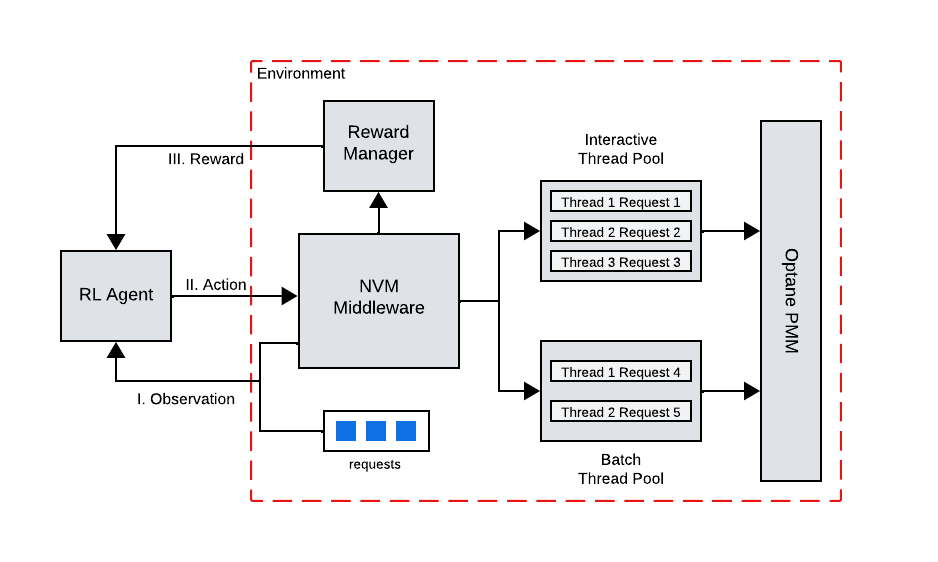
\includegraphics[scale=1]{images/rl_workflow.png}
  \caption[RL Workflow]{RL Workflow}
  \label{fig:rl_workflow}
\end{figure}

Figure \ref{fig:rl_workflow} offers a visual representation of the interaction between the reinforcement learning (RL) agent and the NVM Middleware. At each time step, the NVM Middleware receives a diverse influx of requests, spanning both latency-sensitive and throughput-oriented tasks. These requests necessitate translation into actionable I/O commands directed towards the Intel Optane Persistent Memory Module (PMM).

Concurrently, the RL agent adeptly captures the environment's current state, leveraging real-time workloads' characteristics and performance metrics provided by the monitoring module. Utilizing this information, the agent orchestrates the selection of an optimal action, guiding the dynamic adjustment of threads within the interactive and batch thread pools. This adaptive decision-making process is exemplified by actions like augmenting the count of interactive threads to address evolving workload demands.

Following action selection, the NVM Middleware's resource management module implements the chosen course of action, fine-tuning the NVM Middleware's interactive and batch threads to efficiently handle incoming user requests. Upon the completion of each time step, the action's effectiveness is rigorously assessed against predefined service level agreement (SLA) targets, yielding a reward signal generated by a reward manager.

This reward serves as invaluable feedback for the RL agent, empowering iterative policy updates aimed at refining decision-making strategies in subsequent time steps. Thus, the presented framework embodies a recursive learning cycle, wherein the RL agent continuously hones its behavior through real-world interactions, ensuring adaptive responsiveness to evolving workload dynamics.

\subsection{Reinforcement Learning Model}

\subsubsection{State Space}

\begin{table}[ht]
  \centering
  \caption{The State Representation}
  \label{table:state_space}
  \begin{adjustbox}{width=1\textwidth}
  \begin{tabular}{|l|l|l|}
    \hline
    \thead{Name} & \thead{Description} & \thead{Values} \\
    \hline
    \rowcolor{gray!50}
    interactiveThreads & \makecell[l]{Number of (interactive) threads assigned\\ to the interactive thread pool.} & $1 \leq \text{interactiveThreads} \leq 32$ \\
    \hline
    batchThreads & \makecell[l]{Number of (batch) threads assigned\\ to the batch thread pool.} & $1 \leq \text{batchThreads} \leq 32$ \\
    \hline
    \rowcolor{gray!50}
    interactiveQueueSize & \makecell[l]{Number of requests in the interactive queue.} & $\text{interactiveQueueSize} \in \mathbb{R}^+$ \\
    \hline
    batchQueueSize & \makecell[l]{Number of requests in the batch queue.} & $\text{batchQueueSize} \in \mathbb{R}^+$ \\
    \hline
    \rowcolor{gray!50}
    interactiveBlockSize & \makecell[l]{Average block size of interactive workload.} & $\text{interactiveBlockSize} \in \mathbb{R}^+$ \\
    \hline
    batchBlockSize & \makecell[l]{Average block size of batch workload.} & $\text{batchBlockSize} \in \mathbb{R}^+$ \\
    \hline
    \rowcolor{gray!50}
    interactiveWriteRatio & \makecell[l]{Proportion of write requests compared\\ to read requests in the interactive workload.} & $\text{interactiveRWRatio} \in \mathbb{R}^+$ \\
    \hline
    batchWriteRatio & \makecell[l]{Proportion of write requests compared\\ to read requests in the batch workload.} & $\text{batchRWRatio} \in \mathbb{R}^+$ \\
    \hline
  \end{tabular}
  \end{adjustbox}
\end{table}

Table \ref{table:state_space} presents the features of our state representation. At each time step $t$, we define the state $s_t$ as a tuple:

\[
\begin{aligned}
s_t = (& \text{interactiveThreads}_t, \text{batchThreads}_t, \text{InteractiveQueueSize}_t, \text{batchQueueSize}_t, \\
& \text{interactiveBlockSize}_t, \text{batchBlockSize}_t, \text{interactiveRWRatio}_t, \text{batchRWRatio}_t )
\end{aligned}
\]

where $s_t \in S$ represents the state space. The tuple encapsulates the key features characterizing the system's current state, including the number of interactive and batch threads, number of pending requests in the queues, individual workload block sizes, and write ratio for both interactive and batch workloads.

\subsubsection{Action Space}

\begin{table}[ht]
  \centering
  \caption{Possible Actions in the Action Space}
  \label{table:action_space}
  \begin{tabular}{|c|l|l|}
  \hline
  \thead{Action} & \thead{Effect on \ Interactive Threads} & \thead{Effect on \ Batch Threads} \\
  \hline
  0 & No change & No change \\
  1 & Increase by 1 & No change \\
  2 & Decrease by 1 & No change \\
  3 & No change & Increase by 1 \\
  4 & No change & Decrease by 1 \\
  5 & Increase by 1 & Increase by 1 \\
  6 & Increase by 1 & Decrease by 1 \\
  7 & Decrease by 1 & Increase by 1 \\
  8 & Decrease by 1 & Decrease by 1 \\
  \hline
  \end{tabular}
  \end{table}

  Table \ref{table:action_space} illustrates the feasible actions within the action space. Each action corresponds to a potential adjustment in the number of interactive and batch threads. The table enumerates nine distinct actions, each with its respective effect on the number of interactive threads and batch threads.

  Mathematically, the set of actions $A$ is defined as $A = \{0,1,2,3,4,5,6,7,8\}$ for a given state $s_t \in S$.

\subsubsection{Reward}

\begin{algorithm}[ht]
  % \small
  \caption{Reward Calculation Algorithm}
  \label{algo:reward_calculation}
  \SetAlgoLined
  \KwIn{System statistics: $\text{stat}$}
  \KwOut{Reward value: $\text{reward}$}
  \tcc{Initialize variables}
  $\text{max\_scale\_lat} \leftarrow 1000$, $\text{max\_scale\_tp} \leftarrow 10$, $\text{min\_scale} \leftarrow 1$, $\text{lat\_goal} \leftarrow 200$, $\text{tp\_goal} \leftarrow 250000$, $\text{lat\_penalty} \leftarrow 500.0$, $\text{tp\_penalty} \leftarrow 5000.0$\;
    
  \tcc{Scale observed and target latency and throughput}
  $\text{lat} \leftarrow ((\text{max\_scale\_lat} - \text{min\_scale}) \times (\text{stat.tailLatency} - \text{min\_value}) / (\text{max\_latency} - \text{min\_value})) + \text{min\_scale}$\;
  $\text{tp} \leftarrow ((\text{max\_scale\_tp} - \text{min\_scale}) \times (\text{stat.throughput} - \text{min\_value}) / (\text{max\_throughput} - \text{min\_value})) + \text{min\_scale}$\;
  $\text{lat\_goal} \leftarrow ((\text{max\_scale\_lat} - \text{min\_scale}) \times (\text{lat\_goal} - \text{min\_value}) / (\text{max\_latency} - \text{min\_value})) + \text{min\_scale}$\;
  $\text{tp\_goal} \leftarrow ((\text{max\_scale\_tp} - \text{min\_scale}) \times (\text{tp\_goal} - \text{min\_value}) / (\text{max\_throughput} - \text{min\_value})) + \text{min\_scale}$\;
    
  \tcc{Calculate errors}
  $\text{error\_lat} \leftarrow |\text{lat} - \text{lat\_goal}|$\;
  $\text{error\_tp} \leftarrow |\text{tp} - \text{tp\_goal}|$\;
    
  \tcc{Calculate reward}
  \eIf{$\text{lat} \leq \text{lat\_goal}$ \textbf{and} $\text{tp} \geq \text{tp\_goal}$}{
      $\text{reward} \leftarrow 10 \times (\text{error\_lat} + \text{error\_tp}$) \tcp*{High reward for meeting both latency and throughput goals}
  }{
      \eIf{$\text{lat} > \text{lat\_goal}$ \textbf{and} $\text{tp} < \text{tp\_goal}$}{
          $\text{reward} \leftarrow -1 \times (\text{lat\_penalty} \times \text{error\_lat} + \text{tp\_penalty} \times \text{error\_tp})$ \tcp*{Penalize for high latency and low throughput}
      }{
          \eIf{$\text{lat} > \text{lat\_goal}$}{
              $\text{reward} \leftarrow -1 \times \text{lat\_penalty} \times \text{error\_lat}$ \tcp*{Penalize for high latency}
          }{
              $\text{reward} \leftarrow -1 \times \text{tp\_penalty} \times \text{error\_tp}$ \tcp*{Penalize for low throughput}
          }
      }
  }

\end{algorithm}

To guide the optimization process of the reinforcement learning agent, we establish an algorithm (Algorithm \ref{algo:reward_calculation}) to calculate a reward value based on observed and target latency and throughput metrics. This algorithm, outlined below, serves as a crucial component in training the RL agent to make informed decisions.

\begin{enumerate}
  \item Lines 1-5 define goals, scaling factors, and penalties. The observed and target latency ($lat$, $lat\_goal$) and throughput ($tp$, $tp\_goal$) metrics are scaled to a normalized range using scaling factors ($max\_scale\_lat$, $max\_scale\_tp$) and minimum scale ($min\_scale$). This normalization process ensures that both metrics contribute proportionally to the reward calculation.
  \item Lines 6-7 compare the scaled latency ($lat$) and throughput ($tp$) metrics against the scaled target values for latency ($lat\_goal$) and throughput ($tp\_goal$). The absolute differences between observed and target values are computed to quantify the error in latency ($error\_lat$) and throughput ($error\_tp$).
  \item Lines 8-12 determine the reward based on three distinct scenarios. Firstly, if both latency and throughput goals are achieved, a high positive reward is assigned. Secondly, if both goals are not met, a low negative reward is assigned, taking into account both latency and throughput errors. The disparity in penalties, represented by $lat\_penalty$ and $tp\_penalty$, ensures that both types of errors contribute proportionately to the overall reward. Thirdly, if only the latency goal remains unmet, a low negative reward is assigned, incorporating the latency penalty and error. Finally, if only the throughput goal is unmet, a similar low negative reward is assigned, encompassing the throughput penalty and error.
\end{enumerate}

\subsection{Training Methodology}

\subsubsection{Environment Design}

\begin{figure}[ht]
  \centering
  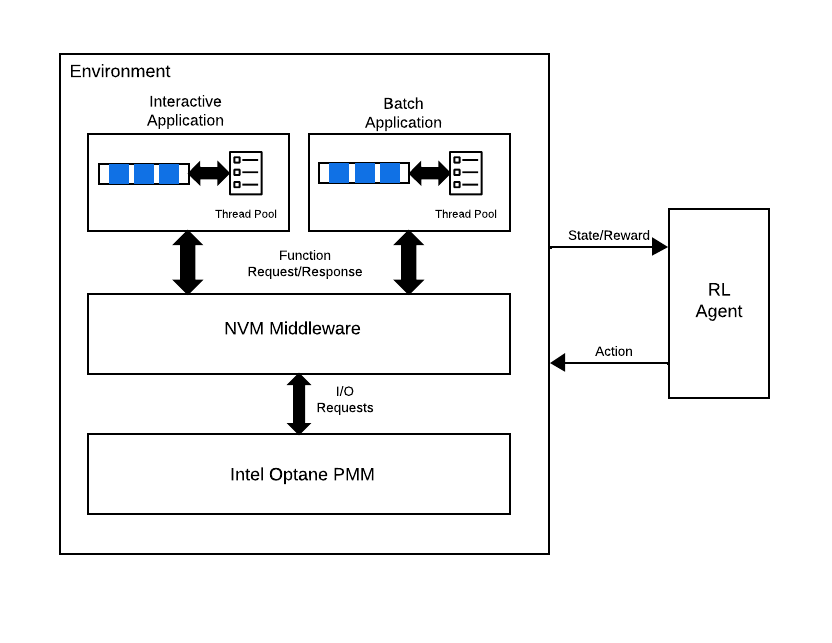
\includegraphics[width=1\textwidth]{images/rl_environment_architecture.png}
  \caption{Overview of the Environment Architecture}
  \label{fig:rl_environment_architecture}
\end{figure}

The environment architecture designed for training and evaluating the RL agent is depicted in Figure \ref{fig:rl_environment_architecture}. This architecture comprises several key components, including an interactive multi-threaded application, a batch multi-threaded application, the NVM Middleware, and Intel Optane PMM.

To simulate a multi-tenant serverless scenario, both applications are executed concurrently. Workload patterns for each application are derived from collected serverless traces. To emulate high concurrency levels typical in serverless environments, multiple threads within each application are employed to dispatch requests to the NVM Middleware via the API described in Section 3.3. Meanwhile, the NVM Middleware processes these requests in accordance with the workflow outlined in Section 3.2.

\begin{figure}[ht]
  \centering
  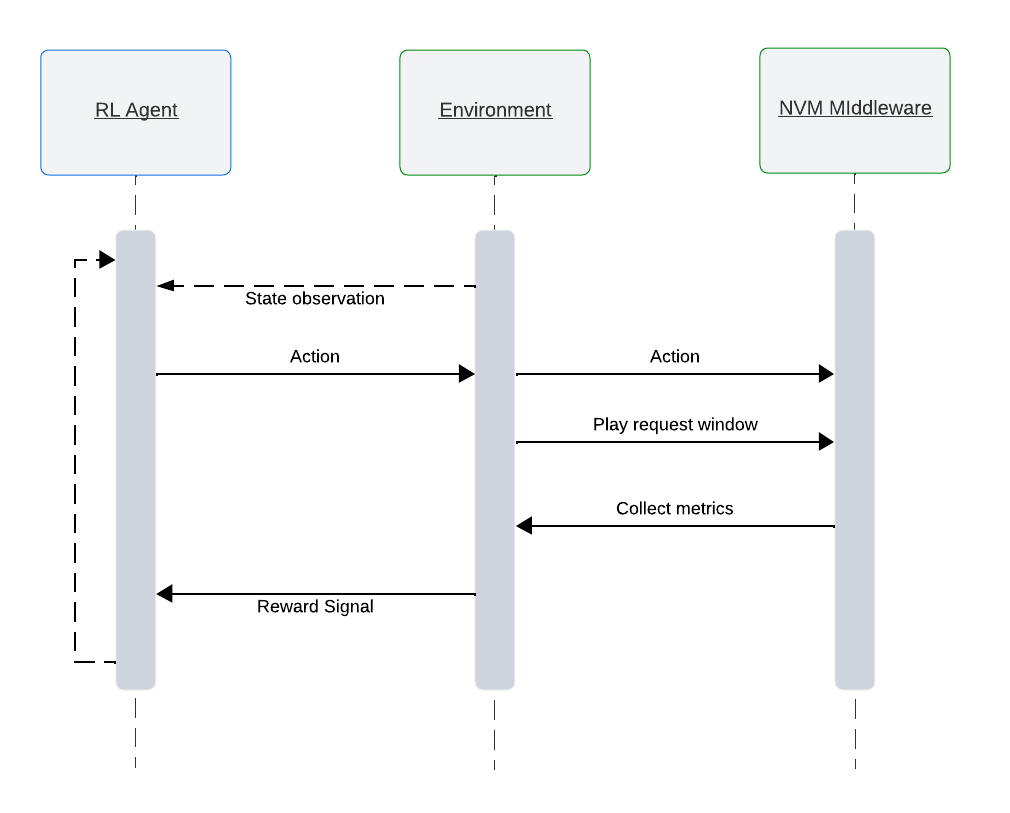
\includegraphics[width=1\textwidth]{images/rl_sequence_flow.png}
  \caption{Agent Process flow}
  \label{fig:rl_sequence_flow}
\end{figure}

In order to model the time steps inherent in an RL process, the environment organizes the applications' requests into 1-second windows, processing one window per time step. Figure \ref{fig:rl_sequence_flow} illustrates the interactions between the RL agent and the environment at each time step. Beginning with a state observation from the preceding step, the agent communicates the intended action to the environment. Subsequently, the environment relays this action to the NVM Middleware, which then allocates resources accordingly. Upon successful execution of the action, the environment initiates processing for the next window of requests. Once all requests within the window are handled, the environment gathers metrics from the NVM Middleware and furnishes a new state observation along with a reward signal to the agent. The agent utilizes this reward to update its policy, perpetuating the iterative learning process.

\subsubsection{Function Approximation}

To address the challenge posed by the continuous state space in our environment, traditional Q-learning approaches become impractical due to the vast number of states that cannot be feasibly mapped into a Q-table. Consequently, we employ function approximation techniques to estimate the value of each action based on the state.

Specifically, we train nine separate linear regression models, each corresponding to one of the available actions, using stochastic gradient descent. This approach allows us to capture the underlying patterns in the data and generalize across states not encountered during training, enabling our agent to make informed decisions even in novel situations.

However, selecting appropriate hyperparameters for our regression models presents a significant challenge. Online training alone is insufficient for accurately assessing model performance, as it can be time-consuming and computationally intensive. To overcome this limitation, we adopt a batch learning approach with offline historical data.

By leveraging historical data collected from the environment, we can tune our models' hyperparameters and incorporate prior knowledge into our RL agent. This approach accelerates the learning process by bootstrapping our models with valuable insights gained from past experiences \cite{cano2017curator,vukosi2015improved}.

To construct our dataset, we deploy a non-optimal agent that performs random actions in the environment, capturing state-action-reward transitions. Following established machine learning practices, we split the dataset into training and testing sets and employ 5-fold cross-validation on the training set to evaluate model performance rigorously.

Additionally, we preprocess the features by standardizing them using the standard scaler and apply polynomial preprocessing to enhance the model's ability to capture nonlinear relationships within the data.


\subsubsection{Proposed Q-Learning Algorithm}

\begin{algorithm}[ht]
  % \small
  \caption{Q-Learning Algorithm}
  \label{algo:q_learning_mw}
  \SetAlgoLined
  \KwIn{Pre-trained Q-value models $M_a$ for all actions $a$}
  \KwOut{Learned Q-value models $M_a$ for all actions $a$}
  Initialize the training parameters $\alpha$, $\gamma$, $\epsilon$\;
  \For{$episode \leftarrow 1$ \KwTo $E$}{
    Reset the environment\;
    \Repeat{episode is done}{
      Observe the state $s_t$\;
      \tcp{Choose action $a_t$ using the $\epsilon$-greedy policy}
      Generate random number $r$ from uniform distribution in [0, 1]\;
      \If{$r < \epsilon$}{
        Select a random action $a_t$ from the action space \;
      }
      \Else{
        \For{each action $a$}{
            Predict Q-value $Q_a(s_t)$ using model $M_a$: $Q_a(s_t) \leftarrow M_a.predict(s_t)$ \;
        }
        Select action $a_t \leftarrow \argmax_a Q_a(s_t)$ \;
      }
      Take action $a_t$, observe reward $r$ and next state $s_{t+1}$\;
      \tcp{Update the Q-value model using reward and next state}
      \If{not done}{
        \For{each action $a$}{
          Predict Q-value $Q_a(s_{t+1})$ using model $M_a$: $Q_a(s_{t+1}) \leftarrow M_a.predict(s_{t+1})$ \;
        }
        Calculate target Q-value: $target \leftarrow r + \gamma \cdot \max_a Q_a(s_{t+1})$ \;
      }
      \Else{
        Set target Q-value to the reward: $target \leftarrow r$ \;
      }
      Update the model for action $a_t$ with the target Q-value: $M_{a_t}.partial\_fit(s_t, target)$ \;
      Update state: $s_t \leftarrow s_{t+1}$\;
    }
    Decrease $\epsilon$ according to exploration schedule\;
  }
\end{algorithm}

Algorithm \ref{algo:q_learning_mw} outlines the Q-Learning process for training an agent to make optimal decisions in an environment. It takes the bootstrapped Q-value models $M_a$ for all actions $a$ and outputs the new learned models after training.

The algorithm initializes the training parameters and then iterates over a specified number of episodes. Within each episode, the environment is reset, and the agent interacts with it until the episode is complete. At each step, the agent observes the current state $s_t$, selects an action $a_t$ based on an $\epsilon$-greedy policy, takes the action, and observes the resulting reward $r$ and next state $s_{t+1}$.

The Q-value models are updated based on the observed reward and next state. If the episode is not done, the target Q-value is calculated using the reward and the maximum Q-value for the next state. If the episode is done, the target Q-value is simply set to the reward.

The model for the selected action $a_t$ is updated using the target Q-value, and the state is updated to the next state. Additionally, the exploration rate $\epsilon$ is decreased according to an exploration schedule.

\section{Implementation}

The NVM Middleware, detailed in Section 3.3, is implemented using C++. We leverage PMEMKV from the Persistent Memory Development Kit \cite{pmdk:book} to facilitate reading and writing data into Intel Optane PMM. To manage concurrent operations efficiently, we utilize the non-locking, concurrent queue provided by the Intel Threading Building Blocks \cite{tbb:online} library for both the interactive and batch queues.

For the RL Environment, as described in Section 3.4.3, we adopt a hybrid approach employing C++ and Python. The environment itself is constructed in C++, aligning with the specifications outlined in Section 3.4.3. Conversely, the RL agent and the Q-Learning algorithm, also discussed in the same section, are developed using Python. We leverage the SGDRegressor model from the Scikit-learn\cite{scikitle61:online} library to facilitate the representation of our linear regression models for function approximation. Additionally, we employ Scikit-learn for hyperparameter tuning. To seamlessly integrate the C++ and Python components, we utilize pybind11\cite{pybind1111:online}.